\documentclass[]{article}
\usepackage{lmodern}
\usepackage{amssymb,amsmath}
\usepackage{ifxetex,ifluatex}
\usepackage{fixltx2e} % provides \textsubscript
\ifnum 0\ifxetex 1\fi\ifluatex 1\fi=0 % if pdftex
  \usepackage[T1]{fontenc}
  \usepackage[utf8]{inputenc}
\else % if luatex or xelatex
  \ifxetex
    \usepackage{mathspec}
  \else
    \usepackage{fontspec}
  \fi
  \defaultfontfeatures{Ligatures=TeX,Scale=MatchLowercase}
\fi
% use upquote if available, for straight quotes in verbatim environments
\IfFileExists{upquote.sty}{\usepackage{upquote}}{}
% use microtype if available
\IfFileExists{microtype.sty}{%
\usepackage{microtype}
\UseMicrotypeSet[protrusion]{basicmath} % disable protrusion for tt fonts
}{}
\usepackage[margin=1in]{geometry}
\usepackage{hyperref}
\hypersetup{unicode=true,
            pdftitle={Tabele Statistice},
            pdfborder={0 0 0},
            breaklinks=true}
\urlstyle{same}  % don't use monospace font for urls
\usepackage{graphicx,grffile}
\makeatletter
\def\maxwidth{\ifdim\Gin@nat@width>\linewidth\linewidth\else\Gin@nat@width\fi}
\def\maxheight{\ifdim\Gin@nat@height>\textheight\textheight\else\Gin@nat@height\fi}
\makeatother
% Scale images if necessary, so that they will not overflow the page
% margins by default, and it is still possible to overwrite the defaults
% using explicit options in \includegraphics[width, height, ...]{}
\setkeys{Gin}{width=\maxwidth,height=\maxheight,keepaspectratio}
\IfFileExists{parskip.sty}{%
\usepackage{parskip}
}{% else
\setlength{\parindent}{0pt}
\setlength{\parskip}{6pt plus 2pt minus 1pt}
}
\setlength{\emergencystretch}{3em}  % prevent overfull lines
\providecommand{\tightlist}{%
  \setlength{\itemsep}{0pt}\setlength{\parskip}{0pt}}
\setcounter{secnumdepth}{5}
% Redefines (sub)paragraphs to behave more like sections
\ifx\paragraph\undefined\else
\let\oldparagraph\paragraph
\renewcommand{\paragraph}[1]{\oldparagraph{#1}\mbox{}}
\fi
\ifx\subparagraph\undefined\else
\let\oldsubparagraph\subparagraph
\renewcommand{\subparagraph}[1]{\oldsubparagraph{#1}\mbox{}}
\fi

%%% Use protect on footnotes to avoid problems with footnotes in titles
\let\rmarkdownfootnote\footnote%
\def\footnote{\protect\rmarkdownfootnote}

%%% Change title format to be more compact
\usepackage{titling}

% Create subtitle command for use in maketitle
\newcommand{\subtitle}[1]{
  \posttitle{
    \begin{center}\large#1\end{center}
    }
}

\setlength{\droptitle}{-2em}
  \title{Tabele Statistice}
  \pretitle{\vspace{\droptitle}\centering\huge}
  \posttitle{\par}
  \author{}
  \preauthor{}\postauthor{}
  \date{}
  \predate{}\postdate{}

\usepackage{booktabs}
\usepackage{longtable}
\usepackage{framed,color}
\definecolor{shadecolor}{RGB}{248, 248, 248}
\definecolor{shadecolor1}{RGB}{216,225,235}
\definecolor{framecolor}{RGB}{108,123,13}

\ifxetex
  \usepackage{letltxmacro}
  \setlength{\XeTeXLinkMargin}{1pt}
  \LetLtxMacro\SavedIncludeGraphics\includegraphics
  \def\includegraphics#1#{% #1 catches optional stuff (star/opt. arg.)
    \IncludeGraphicsAux{#1}%
  }%
  \newcommand*{\IncludeGraphicsAux}[2]{%
    \XeTeXLinkBox{%
      \SavedIncludeGraphics#1{#2}%
    }%
  }%
\fi

\newenvironment{frshaded*}{%
  \def\FrameCommand{\fboxrule=\FrameRule\fboxsep=\FrameSep \fcolorbox{framecolor}{shadecolor1}}%
  \MakeFramed {\advance\hsize-\width \FrameRestore}}%
{\endMakeFramed}

\newenvironment{rmdblock}[1]
  {\begin{frshaded*}
  \begin{itemize}
  \renewcommand{\labelitemi}{
    \raisebox{-.7\height}[0pt][0pt]{
      {\setkeys{Gin}{width=2em,keepaspectratio}\includegraphics{images/icons/#1}}
    }
  }
  \item
  }
  {
  \end{itemize}
  \end{frshaded*}
  }

\newenvironment{rmdcaution}
  {\begin{rmdblock}{caution}}
  {\end{rmdblock}}
% \newenvironment{rmdinsight}
%   {\begin{rmdblock}{insight}}
%   {\end{rmdblock}}
\newenvironment{rmdexercise}
  {\begin{rmdblock}{exercise}}
  {\end{rmdblock}}
\newenvironment{rmdtip}
  {\begin{rmdblock}{tip}}
  {\end{rmdblock}}


%%%%%%%%%%%%%%%%%%%%%%%%%%%%%%%%%%%%%%%%%%%%%%%%%%%%%%%%%%%%%%%%%%%%%%%%%%%%%%%%%%%%%%%%%%%%%%%%%%%%%%%%%%%%%%%%%%%%%
%%%%%%%%%%% For insight block %%%%%%%%%%%%%%%%%%%%%%%%%%
\definecolor{shadecolor_insight}{RGB}{223,240,216}
\definecolor{framecolor_insight}{RGB}{136,193,137}

\newenvironment{frshaded_insight*}{%
  \def\FrameCommand{\fboxrule=\FrameRule\fboxsep=\FrameSep \fcolorbox{framecolor_insight}{shadecolor_insight}}%
  \MakeFramed {\advance\hsize-\width \FrameRestore}}%
{\endMakeFramed}

\newenvironment{rmdblock_insight}[1]
  {\begin{frshaded_insight*}
  \begin{itemize}
  \renewcommand{\labelitemi}{
    \raisebox{-.7\height}[0pt][0pt]{
      {\setkeys{Gin}{width=2em,keepaspectratio}\includegraphics{images/icons/#1}}
    }
  }
  \item
  }
  {
  \end{itemize}
  \end{frshaded_insight*}
  }

\newenvironment{rmdinsight}
  {\begin{rmdblock_insight}{insight}}
  {\end{rmdblock_insight}}

%%%%%%%%%%%%%%%%%%%%%%%%%%%%%%%%%%%%%%%%%%%%%%%%%%%%%%%%%%%%%%%%%%%%%%%%%%%%%%%%%%%%%%%%%%%%%%%%%%%%%%%%%%%%%%%%%%%%%
\usepackage{subfigure}
\usepackage{booktabs}
\usepackage{slashbox}
\usepackage{color}
%%%%%%%%%%%%%%%%%%%%%%%%%%%%%%%%%%%%%%%%%%%%%%%%%%%%%%%%%%%%%%%%%%%%%%%%%%%%%%%%%%%%%%%%%%%%%%%%%%%%%%%%%%%%%%%%%%%%%
%CITEVA DEFINITII
\def\om{\omega}
\def\Om{\Omega}
\def\et{\eta}
\def\td{\tilde{\delta}}
\def\m{{\mu}}
\def\n{{\nu}}
\def\k{{\kappa}}
\def\l{{\lambda}}
\def\L{{\Lambda}}
\def\g{{\gamma}}
\def\a{{\alpha}}
\def\e{{\varepsilon}}
\def\b{{\beta}}
\def\G{{\Gamma}}
\def\d{{\delta}}
\def\D{{\Delta}}
\def\t{{\theta}}
\def\s{{\sigma}}
\def\S{{\Sigma}}
\def\z{{\zeta}}
\def\qed{\hfill\Box}
\def\ds{\displaystyle}
\def\mc{\mathcal}
%%%%%%%%%%%%%%%%%%%%%%%%%%%%%%%%%%%%%%%%%%%%%%%%%%%%%%%%%%%%%%%%%%%%%%%%%%%%%%%%%%%%%%%%%%%%%%%%%%%%%%%%%%%%%%%%%%%%%%
\def\1{{\mathbf 1}}
\def\CC{{\mathbb C}}
\def\VV{{\mathbb V}}
\def\RR{{\mathbb R}}
\def\QQ{{\mathbb Q}}
\def\ZZ{{\mathbb Z}}
\def\PP{{\mathbb P}}
\def\EE{{\mathbb E}}
\def\NN{{\mathbb N}}
\def\FF{{\mathbb F}}
%\def\SS{{\mathbb S}}
\def\MA{{\mathcal A}}
\def\MO{{\mathcal O}}
\def\MF{{\mathcal F}}
\def\ME{{\mathcal E}}
\def\MR{{\mathcal R}}
\def\MB{{\mathcal B}}
\def\MM{{\mathcal M}}
\def\MN{{\mathcal N}}
\def\MU{{\mathcal U}}
\def\MP{{\mathcal P}}
\def\MS{{\mathcal S}}
\def\MBS{{\mathbf S}}
\def\MX{{\bm{ \mathscr X}}}

% independent sign
\newcommand\independent{\protect\mathpalette{\protect\independenT}{\perp}}
\def\independenT#1#2{\mathrel{\rlap{$#1#2$}\mkern2mu{#1#2}}}

%%%%%%%%%%%%%%%%%%%%%%%%%%%%%%%%%%%%%%%%%%%%%%%%%%%%%%%%%%%%%%%%%%%%%%%%%%%%%%%%%%%%%%%%%%%%%%%%%%%%%%%%%%%%%%%%%%%%%
%Header and Footer
\usepackage{fancyhdr}

\pagestyle{fancy}
\fancyhf{}
\rhead{Universitatea din Bucure\c sti\\ Facultatea de Matematic\u a \c si Informatic\u a}
\lhead{\textit{Curs}: Statistic\u a\\ \textit{Instructori}: A. Am\u arioarei, S. Cojocea}
\rfoot{Pagina \thepage}
\lfoot{Grupele: 301, 311, 321}
%%%%%%%%%%%%%%%%%%%%%%%%%%%%%%%%%%%%%%%
\usepackage{booktabs}
\usepackage{longtable}
\usepackage{array}
\usepackage{multirow}
\usepackage[table]{xcolor}
\usepackage{wrapfig}
\usepackage{float}
\usepackage{colortbl}
\usepackage{pdflscape}
\usepackage{tabu}
\usepackage{threeparttable}

\begin{document}
\maketitle

%%%%%%%%%%%%%%%%%%%%%%%%
\thispagestyle{fancy}

În acest document ne propunem să prezentăm mai multe tabele statistice
utile pentru rezolvarea problemelor de probabilități și statistică.

\section{Tabele pentru repartiția normală
standard}\label{tabele-pentru-repartitia-normala-standard}

\subsection{Valorile funcției de
repartiție}\label{valorile-functiei-de-repartitie}

În tabelul următor descriem valorile \textbf{funcției de repartiție},
\(\Phi(x)=\mathbb{P}(X\leq x)\) cu \(x = x_1 + x_2\), pentru o variabilă
aleatoare \(X\) repartizată normal de medie \(0\) și varianță \(1\).
Pentru valori negative putem folosi relația \(\Phi(x) = 1-\Phi(-x)\).

\begin{center}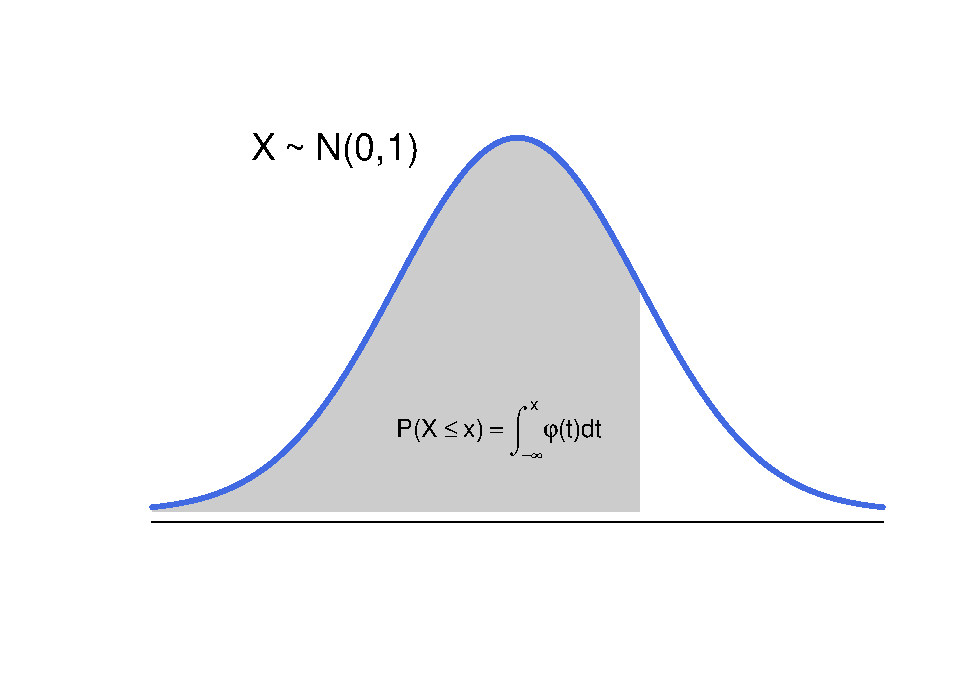
\includegraphics[width=0.4\linewidth]{Tabele_Statistice_files/figure-latex/unnamed-chunk-2-1} \end{center}

\begingroup\fontsize{7}{9}\selectfont
\rowcolors{2}{gray!6}{white}

\begin{longtable}{>{\bfseries}r|rrrrrrrrrr}
\hiderowcolors
\toprule
$x_{1} / x_{2}$ & 0 & 0.01 & 0.02 & 0.03 & 0.04 & 0.05 & 0.06 & 0.07 & 0.08 & 0.09\\
\midrule
\endfirsthead
\multicolumn{11}{@{}l}{\textit{(continued)}}\\
\toprule
$x_{1} / x_{2}$ & 0 & 0.01 & 0.02 & 0.03 & 0.04 & 0.05 & 0.06 & 0.07 & 0.08 & 0.09\\
\midrule
\endhead
\
\endfoot
\bottomrule
\endlastfoot
\showrowcolors
0.0 & 0.5000 & 0.5040 & 0.5080 & 0.5120 & 0.5160 & 0.5199 & 0.5239 & 0.5279 & 0.5319 & 0.5359\\
0.1 & 0.5398 & 0.5438 & 0.5478 & 0.5517 & 0.5557 & 0.5596 & 0.5636 & 0.5675 & 0.5714 & 0.5753\\
0.2 & 0.5793 & 0.5832 & 0.5871 & 0.5910 & 0.5948 & 0.5987 & 0.6026 & 0.6064 & 0.6103 & 0.6141\\
0.3 & 0.6179 & 0.6217 & 0.6255 & 0.6293 & 0.6331 & 0.6368 & 0.6406 & 0.6443 & 0.6480 & 0.6517\\
0.4 & 0.6554 & 0.6591 & 0.6628 & 0.6664 & 0.6700 & 0.6736 & 0.6772 & 0.6808 & 0.6844 & 0.6879\\
\addlinespace
0.5 & 0.6915 & 0.6950 & 0.6985 & 0.7019 & 0.7054 & 0.7088 & 0.7123 & 0.7157 & 0.7190 & 0.7224\\
0.6 & 0.7257 & 0.7291 & 0.7324 & 0.7357 & 0.7389 & 0.7422 & 0.7454 & 0.7486 & 0.7517 & 0.7549\\
0.7 & 0.7580 & 0.7611 & 0.7642 & 0.7673 & 0.7704 & 0.7734 & 0.7764 & 0.7794 & 0.7823 & 0.7852\\
0.8 & 0.7881 & 0.7910 & 0.7939 & 0.7967 & 0.7995 & 0.8023 & 0.8051 & 0.8078 & 0.8106 & 0.8133\\
0.9 & 0.8159 & 0.8186 & 0.8212 & 0.8238 & 0.8264 & 0.8289 & 0.8315 & 0.8340 & 0.8365 & 0.8389\\
\addlinespace
1.0 & 0.8413 & 0.8438 & 0.8461 & 0.8485 & 0.8508 & 0.8531 & 0.8554 & 0.8577 & 0.8599 & 0.8621\\
1.1 & 0.8643 & 0.8665 & 0.8686 & 0.8708 & 0.8729 & 0.8749 & 0.8770 & 0.8790 & 0.8810 & 0.8830\\
1.2 & 0.8849 & 0.8869 & 0.8888 & 0.8907 & 0.8925 & 0.8944 & 0.8962 & 0.8980 & 0.8997 & 0.9015\\
1.3 & 0.9032 & 0.9049 & 0.9066 & 0.9082 & 0.9099 & 0.9115 & 0.9131 & 0.9147 & 0.9162 & 0.9177\\
1.4 & 0.9192 & 0.9207 & 0.9222 & 0.9236 & 0.9251 & 0.9265 & 0.9279 & 0.9292 & 0.9306 & 0.9319\\
\addlinespace
1.5 & 0.9332 & 0.9345 & 0.9357 & 0.9370 & 0.9382 & 0.9394 & 0.9406 & 0.9418 & 0.9429 & 0.9441\\
1.6 & 0.9452 & 0.9463 & 0.9474 & 0.9484 & 0.9495 & 0.9505 & 0.9515 & 0.9525 & 0.9535 & 0.9545\\
1.7 & 0.9554 & 0.9564 & 0.9573 & 0.9582 & 0.9591 & 0.9599 & 0.9608 & 0.9616 & 0.9625 & 0.9633\\
1.8 & 0.9641 & 0.9649 & 0.9656 & 0.9664 & 0.9671 & 0.9678 & 0.9686 & 0.9693 & 0.9699 & 0.9706\\
1.9 & 0.9713 & 0.9719 & 0.9726 & 0.9732 & 0.9738 & 0.9744 & 0.9750 & 0.9756 & 0.9761 & 0.9767\\
\addlinespace
2.0 & 0.9772 & 0.9778 & 0.9783 & 0.9788 & 0.9793 & 0.9798 & 0.9803 & 0.9808 & 0.9812 & 0.9817\\
2.1 & 0.9821 & 0.9826 & 0.9830 & 0.9834 & 0.9838 & 0.9842 & 0.9846 & 0.9850 & 0.9854 & 0.9857\\
2.2 & 0.9861 & 0.9864 & 0.9868 & 0.9871 & 0.9875 & 0.9878 & 0.9881 & 0.9884 & 0.9887 & 0.9890\\
2.3 & 0.9893 & 0.9896 & 0.9898 & 0.9901 & 0.9904 & 0.9906 & 0.9909 & 0.9911 & 0.9913 & 0.9916\\
2.4 & 0.9918 & 0.9920 & 0.9922 & 0.9925 & 0.9927 & 0.9929 & 0.9931 & 0.9932 & 0.9934 & 0.9936\\
\addlinespace
2.5 & 0.9938 & 0.9940 & 0.9941 & 0.9943 & 0.9945 & 0.9946 & 0.9948 & 0.9949 & 0.9951 & 0.9952\\
2.6 & 0.9953 & 0.9955 & 0.9956 & 0.9957 & 0.9959 & 0.9960 & 0.9961 & 0.9962 & 0.9963 & 0.9964\\
2.7 & 0.9965 & 0.9966 & 0.9967 & 0.9968 & 0.9969 & 0.9970 & 0.9971 & 0.9972 & 0.9973 & 0.9974\\
2.8 & 0.9974 & 0.9975 & 0.9976 & 0.9977 & 0.9977 & 0.9978 & 0.9979 & 0.9979 & 0.9980 & 0.9981\\
2.9 & 0.9981 & 0.9982 & 0.9982 & 0.9983 & 0.9984 & 0.9984 & 0.9985 & 0.9985 & 0.9986 & 0.9986\\
3.0 & 0.9987 & 0.9987 & 0.9987 & 0.9988 & 0.9988 & 0.9989 & 0.9989 & 0.9989 & 0.9990 & 0.9990\\*
\end{longtable}

\rowcolors{2}{white}{white}\endgroup{}

\subsection{\texorpdfstring{Cuantilele pentru
\(\mathcal{N}(0,1)\)}{Cuantilele pentru \mathcal\{N\}(0,1)}}\label{cuantilele-pentru-mathcaln01}

În tabelul următor descriem \textbf{cuantilele} de ordin \(\alpha\)
pentru repartiția normală standard, i.e.
\(z_{\alpha}=\Phi^{-1}(\alpha)\) cu \(\alpha = \alpha_1 + \alpha_2\). În
cazul în care \(\alpha<0.5\) vom folosi relația
\(z_{\alpha} = -z_{1-\alpha}\).

\begin{center}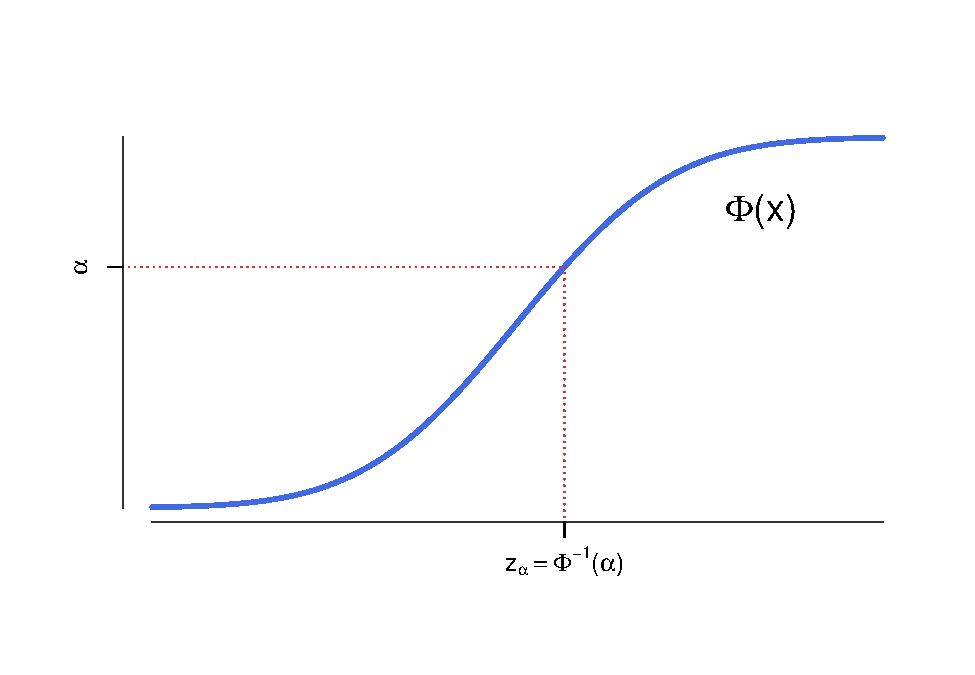
\includegraphics[width=0.4\linewidth]{Tabele_Statistice_files/figure-latex/unnamed-chunk-4-1} \end{center}

\begingroup\fontsize{7}{9}\selectfont
\rowcolors{2}{gray!6}{white}

\begin{longtable}{>{\bfseries}r|rrrrrrrrrr}
\hiderowcolors
\toprule
$\alpha_{1} / \alpha_{2}$ & 0 & 0.001 & 0.002 & 0.003 & 0.004 & 0.005 & 0.006 & 0.007 & 0.008 & 0.009\\
\midrule
\endfirsthead
\multicolumn{11}{@{}l}{\textit{(continued)}}\\
\toprule
$\alpha_{1} / \alpha_{2}$ & 0 & 0.001 & 0.002 & 0.003 & 0.004 & 0.005 & 0.006 & 0.007 & 0.008 & 0.009\\
\midrule
\endhead
\
\endfoot
\bottomrule
\endlastfoot
\showrowcolors
0.50 & 0.0000 & 0.0025 & 0.0050 & 0.0075 & 0.0100 & 0.0125 & 0.0150 & 0.0175 & 0.0201 & 0.0226\\
0.51 & 0.0251 & 0.0276 & 0.0301 & 0.0326 & 0.0351 & 0.0376 & 0.0401 & 0.0426 & 0.0451 & 0.0476\\
0.52 & 0.0502 & 0.0527 & 0.0552 & 0.0577 & 0.0602 & 0.0627 & 0.0652 & 0.0677 & 0.0702 & 0.0728\\
0.53 & 0.0753 & 0.0778 & 0.0803 & 0.0828 & 0.0853 & 0.0878 & 0.0904 & 0.0929 & 0.0954 & 0.0979\\
0.54 & 0.1004 & 0.1030 & 0.1055 & 0.1080 & 0.1105 & 0.1130 & 0.1156 & 0.1181 & 0.1206 & 0.1231\\
\addlinespace
0.55 & 0.1257 & 0.1282 & 0.1307 & 0.1332 & 0.1358 & 0.1383 & 0.1408 & 0.1434 & 0.1459 & 0.1484\\
0.56 & 0.1510 & 0.1535 & 0.1560 & 0.1586 & 0.1611 & 0.1637 & 0.1662 & 0.1687 & 0.1713 & 0.1738\\
0.57 & 0.1764 & 0.1789 & 0.1815 & 0.1840 & 0.1866 & 0.1891 & 0.1917 & 0.1942 & 0.1968 & 0.1993\\
0.58 & 0.2019 & 0.2045 & 0.2070 & 0.2096 & 0.2121 & 0.2147 & 0.2173 & 0.2198 & 0.2224 & 0.2250\\
0.59 & 0.2275 & 0.2301 & 0.2327 & 0.2353 & 0.2378 & 0.2404 & 0.2430 & 0.2456 & 0.2482 & 0.2508\\
\addlinespace
0.60 & 0.2533 & 0.2559 & 0.2585 & 0.2611 & 0.2637 & 0.2663 & 0.2689 & 0.2715 & 0.2741 & 0.2767\\
0.61 & 0.2793 & 0.2819 & 0.2845 & 0.2871 & 0.2898 & 0.2924 & 0.2950 & 0.2976 & 0.3002 & 0.3029\\
0.62 & 0.3055 & 0.3081 & 0.3107 & 0.3134 & 0.3160 & 0.3186 & 0.3213 & 0.3239 & 0.3266 & 0.3292\\
0.63 & 0.3319 & 0.3345 & 0.3372 & 0.3398 & 0.3425 & 0.3451 & 0.3478 & 0.3505 & 0.3531 & 0.3558\\
0.64 & 0.3585 & 0.3611 & 0.3638 & 0.3665 & 0.3692 & 0.3719 & 0.3745 & 0.3772 & 0.3799 & 0.3826\\
\addlinespace
0.65 & 0.3853 & 0.3880 & 0.3907 & 0.3934 & 0.3961 & 0.3989 & 0.4016 & 0.4043 & 0.4070 & 0.4097\\
0.66 & 0.4125 & 0.4152 & 0.4179 & 0.4207 & 0.4234 & 0.4261 & 0.4289 & 0.4316 & 0.4344 & 0.4372\\
0.67 & 0.4399 & 0.4427 & 0.4454 & 0.4482 & 0.4510 & 0.4538 & 0.4565 & 0.4593 & 0.4621 & 0.4649\\
0.68 & 0.4677 & 0.4705 & 0.4733 & 0.4761 & 0.4789 & 0.4817 & 0.4845 & 0.4874 & 0.4902 & 0.4930\\
0.69 & 0.4959 & 0.4987 & 0.5015 & 0.5044 & 0.5072 & 0.5101 & 0.5129 & 0.5158 & 0.5187 & 0.5215\\
\addlinespace
0.70 & 0.5244 & 0.5273 & 0.5302 & 0.5330 & 0.5359 & 0.5388 & 0.5417 & 0.5446 & 0.5476 & 0.5505\\
0.71 & 0.5534 & 0.5563 & 0.5592 & 0.5622 & 0.5651 & 0.5681 & 0.5710 & 0.5740 & 0.5769 & 0.5799\\
0.72 & 0.5828 & 0.5858 & 0.5888 & 0.5918 & 0.5948 & 0.5978 & 0.6008 & 0.6038 & 0.6068 & 0.6098\\
0.73 & 0.6128 & 0.6158 & 0.6189 & 0.6219 & 0.6250 & 0.6280 & 0.6311 & 0.6341 & 0.6372 & 0.6403\\
0.74 & 0.6433 & 0.6464 & 0.6495 & 0.6526 & 0.6557 & 0.6588 & 0.6620 & 0.6651 & 0.6682 & 0.6713\\
\addlinespace
0.75 & 0.6745 & 0.6776 & 0.6808 & 0.6840 & 0.6871 & 0.6903 & 0.6935 & 0.6967 & 0.6999 & 0.7031\\
0.76 & 0.7063 & 0.7095 & 0.7128 & 0.7160 & 0.7192 & 0.7225 & 0.7257 & 0.7290 & 0.7323 & 0.7356\\
0.77 & 0.7388 & 0.7421 & 0.7454 & 0.7488 & 0.7521 & 0.7554 & 0.7588 & 0.7621 & 0.7655 & 0.7688\\
0.78 & 0.7722 & 0.7756 & 0.7790 & 0.7824 & 0.7858 & 0.7892 & 0.7926 & 0.7961 & 0.7995 & 0.8030\\
0.79 & 0.8064 & 0.8099 & 0.8134 & 0.8169 & 0.8204 & 0.8239 & 0.8274 & 0.8310 & 0.8345 & 0.8381\\
\addlinespace
0.80 & 0.8416 & 0.8452 & 0.8488 & 0.8524 & 0.8560 & 0.8596 & 0.8633 & 0.8669 & 0.8705 & 0.8742\\
0.81 & 0.8779 & 0.8816 & 0.8853 & 0.8890 & 0.8927 & 0.8965 & 0.9002 & 0.9040 & 0.9078 & 0.9116\\
0.82 & 0.9154 & 0.9192 & 0.9230 & 0.9269 & 0.9307 & 0.9346 & 0.9385 & 0.9424 & 0.9463 & 0.9502\\
0.83 & 0.9542 & 0.9581 & 0.9621 & 0.9661 & 0.9701 & 0.9741 & 0.9782 & 0.9822 & 0.9863 & 0.9904\\
0.84 & 0.9945 & 0.9986 & 1.0027 & 1.0069 & 1.0110 & 1.0152 & 1.0194 & 1.0237 & 1.0279 & 1.0322\\
\addlinespace
0.85 & 1.0364 & 1.0407 & 1.0450 & 1.0494 & 1.0537 & 1.0581 & 1.0625 & 1.0669 & 1.0714 & 1.0758\\
0.86 & 1.0803 & 1.0848 & 1.0893 & 1.0939 & 1.0985 & 1.1031 & 1.1077 & 1.1123 & 1.1170 & 1.1217\\
0.87 & 1.1264 & 1.1311 & 1.1359 & 1.1407 & 1.1455 & 1.1503 & 1.1552 & 1.1601 & 1.1650 & 1.1700\\
0.88 & 1.1750 & 1.1800 & 1.1850 & 1.1901 & 1.1952 & 1.2004 & 1.2055 & 1.2107 & 1.2160 & 1.2212\\
0.89 & 1.2265 & 1.2319 & 1.2372 & 1.2426 & 1.2481 & 1.2536 & 1.2591 & 1.2646 & 1.2702 & 1.2759\\
\addlinespace
0.90 & 1.2816 & 1.2873 & 1.2930 & 1.2988 & 1.3047 & 1.3106 & 1.3165 & 1.3225 & 1.3285 & 1.3346\\
0.91 & 1.3408 & 1.3469 & 1.3532 & 1.3595 & 1.3658 & 1.3722 & 1.3787 & 1.3852 & 1.3917 & 1.3984\\
0.92 & 1.4051 & 1.4118 & 1.4187 & 1.4255 & 1.4325 & 1.4395 & 1.4466 & 1.4538 & 1.4611 & 1.4684\\
0.93 & 1.4758 & 1.4833 & 1.4909 & 1.4985 & 1.5063 & 1.5141 & 1.5220 & 1.5301 & 1.5382 & 1.5464\\
0.94 & 1.5548 & 1.5632 & 1.5718 & 1.5805 & 1.5893 & 1.5982 & 1.6072 & 1.6164 & 1.6258 & 1.6352\\
\addlinespace
0.95 & 1.6449 & 1.6546 & 1.6646 & 1.6747 & 1.6849 & 1.6954 & 1.7060 & 1.7169 & 1.7279 & 1.7392\\
0.96 & 1.7507 & 1.7624 & 1.7744 & 1.7866 & 1.7991 & 1.8119 & 1.8250 & 1.8384 & 1.8522 & 1.8663\\
0.97 & 1.8808 & 1.8957 & 1.9110 & 1.9268 & 1.9431 & 1.9600 & 1.9774 & 1.9954 & 2.0141 & 2.0335\\
0.98 & 2.0537 & 2.0749 & 2.0969 & 2.1201 & 2.1444 & 2.1701 & 2.1973 & 2.2262 & 2.2571 & 2.2904\\
0.99 & 2.3263 & 2.3656 & 2.4089 & 2.4573 & 2.5121 & 2.5758 & 2.6521 & 2.7478 & 2.8782 & 3.0902\\*
\end{longtable}

\rowcolors{2}{white}{white}\endgroup{}

\section{Tabel pentru repartiția
t-Student}\label{tabel-pentru-repartitia-t-student}

Tabelul următor prezintă cuantilele de ordin \(\alpha\) pentru repatiția
t-Student cu \(\nu\) grade de libertate. Pentru valori ale lui
\(\alpha\leq 0.5\) se poate folosi relația următoare
\(t_{\nu,\alpha} = - t_{\nu,1-\alpha}\).

\begin{center}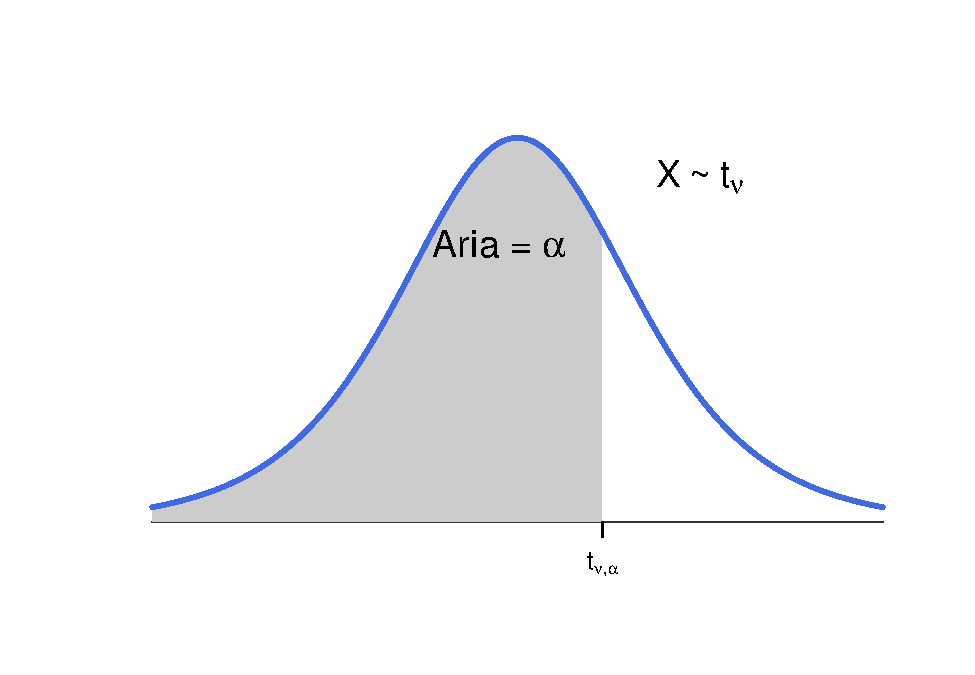
\includegraphics[width=0.4\linewidth]{Tabele_Statistice_files/figure-latex/unnamed-chunk-6-1} \end{center}

\begingroup\fontsize{7}{9}\selectfont
\rowcolors{2}{gray!6}{white}

\begin{longtable}{>{\bfseries}r|rrrrrrrr}
\hiderowcolors
\toprule
$\nu / \alpha$ & 0.6 & 0.75 & 0.9 & 0.95 & 0.975 & 0.99 & 0.995 & 0.9995\\
\midrule
\endfirsthead
\multicolumn{9}{@{}l}{\textit{(continued)}}\\
\toprule
$\nu / \alpha$ & 0.6 & 0.75 & 0.9 & 0.95 & 0.975 & 0.99 & 0.995 & 0.9995\\
\midrule
\endhead
\
\endfoot
\bottomrule
\endlastfoot
\showrowcolors
1 & 0.3249 & 1.0000 & 3.078 & 6.314 & 12.706 & 31.820 & 63.657 & 636.619\\
2 & 0.2887 & 0.8165 & 1.886 & 2.920 & 4.303 & 6.965 & 9.925 & 31.599\\
3 & 0.2767 & 0.7649 & 1.638 & 2.353 & 3.182 & 4.541 & 5.841 & 12.924\\
4 & 0.2707 & 0.7407 & 1.533 & 2.132 & 2.776 & 3.747 & 4.604 & 8.610\\
5 & 0.2672 & 0.7267 & 1.476 & 2.015 & 2.571 & 3.365 & 4.032 & 6.869\\
\addlinespace
6 & 0.2648 & 0.7176 & 1.440 & 1.943 & 2.447 & 3.143 & 3.707 & 5.959\\
7 & 0.2632 & 0.7111 & 1.415 & 1.895 & 2.365 & 2.998 & 3.499 & 5.408\\
8 & 0.2619 & 0.7064 & 1.397 & 1.859 & 2.306 & 2.897 & 3.355 & 5.041\\
9 & 0.2610 & 0.7027 & 1.383 & 1.833 & 2.262 & 2.821 & 3.250 & 4.781\\
10 & 0.2602 & 0.6998 & 1.372 & 1.812 & 2.228 & 2.764 & 3.169 & 4.587\\
\addlinespace
11 & 0.2596 & 0.6974 & 1.363 & 1.796 & 2.201 & 2.718 & 3.106 & 4.437\\
12 & 0.2590 & 0.6955 & 1.356 & 1.782 & 2.179 & 2.681 & 3.054 & 4.318\\
13 & 0.2586 & 0.6938 & 1.350 & 1.771 & 2.160 & 2.650 & 3.012 & 4.221\\
14 & 0.2582 & 0.6924 & 1.345 & 1.761 & 2.145 & 2.624 & 2.977 & 4.141\\
15 & 0.2579 & 0.6912 & 1.341 & 1.753 & 2.131 & 2.603 & 2.947 & 4.073\\
\addlinespace
16 & 0.2576 & 0.6901 & 1.337 & 1.746 & 2.120 & 2.583 & 2.921 & 4.015\\
17 & 0.2573 & 0.6892 & 1.333 & 1.740 & 2.110 & 2.567 & 2.898 & 3.965\\
18 & 0.2571 & 0.6884 & 1.330 & 1.734 & 2.101 & 2.552 & 2.878 & 3.922\\
19 & 0.2569 & 0.6876 & 1.328 & 1.729 & 2.093 & 2.539 & 2.861 & 3.883\\
20 & 0.2567 & 0.6870 & 1.325 & 1.725 & 2.086 & 2.528 & 2.845 & 3.849\\
\addlinespace
21 & 0.2566 & 0.6864 & 1.323 & 1.721 & 2.080 & 2.518 & 2.831 & 3.819\\
22 & 0.2564 & 0.6858 & 1.321 & 1.717 & 2.074 & 2.508 & 2.819 & 3.792\\
23 & 0.2563 & 0.6853 & 1.319 & 1.714 & 2.069 & 2.500 & 2.807 & 3.768\\
24 & 0.2562 & 0.6848 & 1.318 & 1.711 & 2.064 & 2.492 & 2.797 & 3.745\\
25 & 0.2561 & 0.6844 & 1.316 & 1.708 & 2.059 & 2.485 & 2.787 & 3.725\\
\addlinespace
26 & 0.2560 & 0.6840 & 1.315 & 1.706 & 2.055 & 2.479 & 2.779 & 3.707\\
27 & 0.2559 & 0.6837 & 1.314 & 1.703 & 2.052 & 2.473 & 2.771 & 3.690\\
28 & 0.2558 & 0.6834 & 1.312 & 1.701 & 2.048 & 2.467 & 2.763 & 3.674\\
29 & 0.2557 & 0.6830 & 1.311 & 1.699 & 2.045 & 2.462 & 2.756 & 3.659\\
30 & 0.2556 & 0.6828 & 1.310 & 1.697 & 2.042 & 2.457 & 2.750 & 3.646\\
\addlinespace
40 & 0.2550 & 0.6807 & 1.303 & 1.684 & 2.021 & 2.423 & 2.704 & 3.551\\
60 & 0.2545 & 0.6786 & 1.296 & 1.671 & 2.000 & 2.390 & 2.660 & 3.460\\
120 & 0.2539 & 0.6765 & 1.289 & 1.658 & 1.980 & 2.358 & 2.617 & 3.373\\
1000 & 0.2534 & 0.6747 & 1.282 & 1.646 & 1.962 & 2.330 & 2.581 & 3.300\\*
\end{longtable}

\rowcolors{2}{white}{white}\endgroup{}

\section{\texorpdfstring{Tabel pentru repartiția
\(\chi^2\)}{Tabel pentru repartiția \chi\^{}2}}\label{tabel-pentru-repartitia-chi2}

Tabelul de mai jos prezintă cuantilele de ordin \(\alpha\) ale
repartiției \(\chi^2_{\nu}\). Dacă \(X\sim \chi^2_{\nu}\) atunci
\(\mathbb{E}[X]=\nu\) și \(Var(X) = 2\nu\). Pentru valori \(\nu>50\) vom
folosi formula
\(\chi^2_{\nu,\alpha} \approx \frac{(z_{\alpha}+\sqrt{2\nu-1})^2}{2}\)
pentru a aproxima cuantilele repartiției \(\chi^2_{\nu}\), unde
\(z_{\alpha}\) este cuantila de ordin \(\alpha\) a repartiției normale
standard.

\begin{center}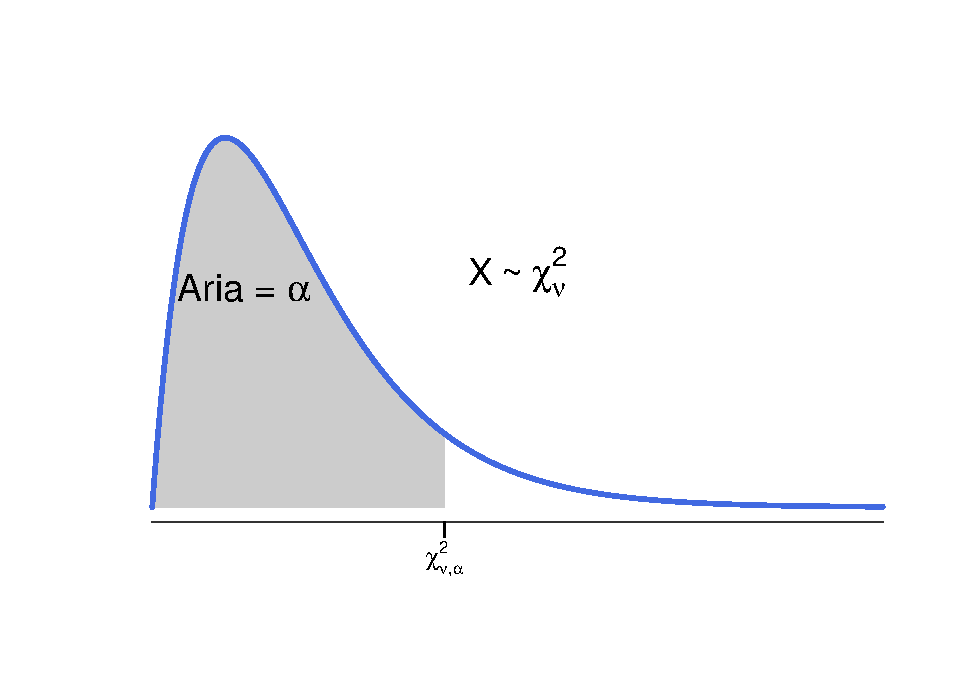
\includegraphics[width=0.4\linewidth]{Tabele_Statistice_files/figure-latex/unnamed-chunk-8-1} \end{center}

\begingroup\fontsize{6}{8}\selectfont
\rowcolors{2}{gray!6}{white}

\begin{longtable}{>{\bfseries}r|rrrrrrrrrrrrr}
\hiderowcolors
\toprule
$\nu / \alpha$ & 0.005 & 0.01 & 0.025 & 0.05 & 0.1 & 0.25 & 0.5 & 0.75 & 0.9 & 0.95 & 0.975 & 0.99 & 0.995\\
\midrule
\endfirsthead
\multicolumn{14}{@{}l}{\textit{(continued)}}\\
\toprule
$\nu / \alpha$ & 0.005 & 0.01 & 0.025 & 0.05 & 0.1 & 0.25 & 0.5 & 0.75 & 0.9 & 0.95 & 0.975 & 0.99 & 0.995\\
\midrule
\endhead
\
\endfoot
\bottomrule
\endlastfoot
\showrowcolors
1 & 0.0000 & 0.0002 & 0.0010 & 0.0039 & 0.0158 & 0.1015 & 0.4549 & 1.323 & 2.705 & 3.841 & 5.024 & 6.635 & 7.879\\
2 & 0.0100 & 0.0201 & 0.0506 & 0.1026 & 0.2107 & 0.5754 & 1.3863 & 2.773 & 4.605 & 5.992 & 7.378 & 9.210 & 10.597\\
3 & 0.0717 & 0.1148 & 0.2158 & 0.3518 & 0.5844 & 1.2125 & 2.3660 & 4.108 & 6.251 & 7.815 & 9.348 & 11.345 & 12.838\\
4 & 0.2070 & 0.2971 & 0.4844 & 0.7107 & 1.0636 & 1.9226 & 3.3567 & 5.385 & 7.779 & 9.488 & 11.143 & 13.277 & 14.860\\
5 & 0.4117 & 0.5543 & 0.8312 & 1.1455 & 1.6103 & 2.6746 & 4.3515 & 6.626 & 9.236 & 11.070 & 12.832 & 15.086 & 16.750\\
\addlinespace
6 & 0.6757 & 0.8721 & 1.2373 & 1.6354 & 2.2041 & 3.4546 & 5.3481 & 7.841 & 10.645 & 12.592 & 14.449 & 16.812 & 18.548\\
7 & 0.9893 & 1.2390 & 1.6899 & 2.1673 & 2.8331 & 4.2549 & 6.3458 & 9.037 & 12.017 & 14.067 & 16.013 & 18.475 & 20.278\\
8 & 1.3444 & 1.6465 & 2.1797 & 2.7326 & 3.4895 & 5.0706 & 7.3441 & 10.219 & 13.362 & 15.507 & 17.535 & 20.090 & 21.955\\
9 & 1.7349 & 2.0879 & 2.7004 & 3.3251 & 4.1682 & 5.8988 & 8.3428 & 11.389 & 14.684 & 16.919 & 19.023 & 21.666 & 23.589\\
10 & 2.1559 & 2.5582 & 3.2470 & 3.9403 & 4.8652 & 6.7372 & 9.3418 & 12.549 & 15.987 & 18.307 & 20.483 & 23.209 & 25.188\\
\addlinespace
11 & 2.6032 & 3.0535 & 3.8157 & 4.5748 & 5.5778 & 7.5841 & 10.3410 & 13.701 & 17.275 & 19.675 & 21.920 & 24.725 & 26.757\\
12 & 3.0738 & 3.5706 & 4.4038 & 5.2260 & 6.3038 & 8.4384 & 11.3403 & 14.845 & 18.549 & 21.026 & 23.337 & 26.217 & 28.299\\
13 & 3.5650 & 4.1069 & 5.0088 & 5.8919 & 7.0415 & 9.2991 & 12.3398 & 15.984 & 19.812 & 22.362 & 24.736 & 27.688 & 29.820\\
14 & 4.0747 & 4.6604 & 5.6287 & 6.5706 & 7.7895 & 10.1653 & 13.3393 & 17.117 & 21.064 & 23.685 & 26.119 & 29.141 & 31.319\\
15 & 4.6009 & 5.2293 & 6.2621 & 7.2609 & 8.5468 & 11.0365 & 14.3389 & 18.245 & 22.307 & 24.996 & 27.488 & 30.578 & 32.801\\
\addlinespace
16 & 5.1422 & 5.8122 & 6.9077 & 7.9616 & 9.3122 & 11.9122 & 15.3385 & 19.369 & 23.542 & 26.296 & 28.845 & 32.000 & 34.267\\
17 & 5.6972 & 6.4078 & 7.5642 & 8.6718 & 10.0852 & 12.7919 & 16.3382 & 20.489 & 24.769 & 27.587 & 30.191 & 33.409 & 35.718\\
18 & 6.2648 & 7.0149 & 8.2307 & 9.3905 & 10.8649 & 13.6753 & 17.3379 & 21.605 & 25.989 & 28.869 & 31.526 & 34.805 & 37.157\\
19 & 6.8440 & 7.6327 & 8.9065 & 10.1170 & 11.6509 & 14.5620 & 18.3377 & 22.718 & 27.204 & 30.143 & 32.852 & 36.191 & 38.582\\
20 & 7.4338 & 8.2604 & 9.5908 & 10.8508 & 12.4426 & 15.4518 & 19.3374 & 23.828 & 28.412 & 31.410 & 34.170 & 37.566 & 39.997\\
\addlinespace
21 & 8.0337 & 8.8972 & 10.2829 & 11.5913 & 13.2396 & 16.3444 & 20.3372 & 24.935 & 29.615 & 32.671 & 35.479 & 38.932 & 41.401\\
22 & 8.6427 & 9.5425 & 10.9823 & 12.3380 & 14.0415 & 17.2396 & 21.3370 & 26.039 & 30.813 & 33.924 & 36.781 & 40.289 & 42.796\\
23 & 9.2604 & 10.1957 & 11.6886 & 13.0905 & 14.8480 & 18.1373 & 22.3369 & 27.141 & 32.007 & 35.172 & 38.076 & 41.638 & 44.181\\
24 & 9.8862 & 10.8564 & 12.4012 & 13.8484 & 15.6587 & 19.0373 & 23.3367 & 28.241 & 33.196 & 36.415 & 39.364 & 42.980 & 45.559\\
25 & 10.5197 & 11.5240 & 13.1197 & 14.6114 & 16.4734 & 19.9393 & 24.3366 & 29.339 & 34.382 & 37.653 & 40.647 & 44.314 & 46.928\\
\addlinespace
26 & 11.1602 & 12.1981 & 13.8439 & 15.3792 & 17.2919 & 20.8434 & 25.3365 & 30.435 & 35.563 & 38.885 & 41.923 & 45.642 & 48.290\\
27 & 11.8076 & 12.8785 & 14.5734 & 16.1514 & 18.1139 & 21.7494 & 26.3363 & 31.528 & 36.741 & 40.113 & 43.194 & 46.963 & 49.645\\
28 & 12.4613 & 13.5647 & 15.3079 & 16.9279 & 18.9392 & 22.6572 & 27.3362 & 32.620 & 37.916 & 41.337 & 44.461 & 48.278 & 50.993\\
29 & 13.1211 & 14.2565 & 16.0471 & 17.7084 & 19.7677 & 23.5666 & 28.3361 & 33.711 & 39.087 & 42.557 & 45.722 & 49.588 & 52.336\\
30 & 13.7867 & 14.9535 & 16.7908 & 18.4927 & 20.5992 & 24.4776 & 29.3360 & 34.800 & 40.256 & 43.773 & 46.979 & 50.892 & 53.672\\
\addlinespace
31 & 14.4578 & 15.6555 & 17.5387 & 19.2806 & 21.4336 & 25.3901 & 30.3359 & 35.887 & 41.422 & 44.985 & 48.232 & 52.191 & 55.003\\
32 & 15.1340 & 16.3622 & 18.2908 & 20.0719 & 22.2706 & 26.3041 & 31.3359 & 36.973 & 42.585 & 46.194 & 49.480 & 53.486 & 56.328\\
33 & 15.8153 & 17.0735 & 19.0467 & 20.8665 & 23.1102 & 27.2194 & 32.3358 & 38.057 & 43.745 & 47.400 & 50.725 & 54.776 & 57.648\\
34 & 16.5013 & 17.7891 & 19.8063 & 21.6643 & 23.9523 & 28.1361 & 33.3357 & 39.141 & 44.903 & 48.602 & 51.966 & 56.061 & 58.964\\
35 & 17.1918 & 18.5089 & 20.5694 & 22.4650 & 24.7967 & 29.0540 & 34.3356 & 40.223 & 46.059 & 49.802 & 53.203 & 57.342 & 60.275\\
\addlinespace
36 & 17.8867 & 19.2327 & 21.3359 & 23.2686 & 25.6433 & 29.9730 & 35.3356 & 41.304 & 47.212 & 50.998 & 54.437 & 58.619 & 61.581\\
37 & 18.5858 & 19.9602 & 22.1056 & 24.0749 & 26.4921 & 30.8933 & 36.3355 & 42.383 & 48.363 & 52.192 & 55.668 & 59.892 & 62.883\\
38 & 19.2889 & 20.6914 & 22.8785 & 24.8839 & 27.3430 & 31.8146 & 37.3355 & 43.462 & 49.513 & 53.383 & 56.895 & 61.162 & 64.181\\
39 & 19.9959 & 21.4262 & 23.6543 & 25.6954 & 28.1958 & 32.7369 & 38.3354 & 44.539 & 50.660 & 54.572 & 58.120 & 62.428 & 65.476\\
40 & 20.7065 & 22.1643 & 24.4330 & 26.5093 & 29.0505 & 33.6603 & 39.3353 & 45.616 & 51.805 & 55.758 & 59.342 & 63.691 & 66.766\\
\addlinespace
41 & 21.4208 & 22.9056 & 25.2145 & 27.3256 & 29.9071 & 34.5846 & 40.3353 & 46.692 & 52.949 & 56.942 & 60.561 & 64.950 & 68.053\\
42 & 22.1385 & 23.6501 & 25.9987 & 28.1440 & 30.7654 & 35.5099 & 41.3352 & 47.766 & 54.090 & 58.124 & 61.777 & 66.206 & 69.336\\
43 & 22.8595 & 24.3976 & 26.7854 & 28.9647 & 31.6255 & 36.4361 & 42.3352 & 48.840 & 55.230 & 59.303 & 62.990 & 67.459 & 70.616\\
44 & 23.5837 & 25.1480 & 27.5746 & 29.7875 & 32.4871 & 37.3631 & 43.3352 & 49.913 & 56.368 & 60.481 & 64.201 & 68.710 & 71.893\\
45 & 24.3110 & 25.9013 & 28.3662 & 30.6123 & 33.3504 & 38.2910 & 44.3351 & 50.985 & 57.505 & 61.656 & 65.410 & 69.957 & 73.166\\
\addlinespace
46 & 25.0413 & 26.6572 & 29.1601 & 31.4390 & 34.2152 & 39.2197 & 45.3351 & 52.056 & 58.641 & 62.830 & 66.617 & 71.201 & 74.436\\
47 & 25.7746 & 27.4158 & 29.9562 & 32.2676 & 35.0814 & 40.1492 & 46.3350 & 53.127 & 59.774 & 64.001 & 67.821 & 72.443 & 75.704\\
48 & 26.5106 & 28.1770 & 30.7545 & 33.0981 & 35.9491 & 41.0794 & 47.3350 & 54.196 & 60.907 & 65.171 & 69.023 & 73.683 & 76.969\\
49 & 27.2493 & 28.9406 & 31.5549 & 33.9303 & 36.8182 & 42.0104 & 48.3350 & 55.265 & 62.038 & 66.339 & 70.222 & 74.919 & 78.231\\
50 & 27.9907 & 29.7067 & 32.3574 & 34.7643 & 37.6886 & 42.9421 & 49.3349 & 56.334 & 63.167 & 67.505 & 71.420 & 76.154 & 79.490\\*
\end{longtable}

\rowcolors{2}{white}{white}\endgroup{}

\section{Tabel pentru repartiția
Fischer-Snedecor}\label{tabel-pentru-repartitia-fischer-snedecor}

Tabelele care urmează prezintă cuantilele de ordin
\(\alpha\in\{0.9, 0.95, 0.975\}\) pentru repartiția Fischer-Snedecor cu
\(\nu_1\) grade de libertate la numărător și \(\nu_2\) grade de
libertate la numitor. Pentru valori ale lui \(\alpha \leq 0.5\) se poate
folosi relația
\(F_{\nu_1, \nu_2, \alpha} = \frac{1}{F_{\nu_2, \nu_1, 1-\alpha}}\).

\subsection{\texorpdfstring{Cunatile pentru
\(F_{\nu_1, \nu_2, 0.9}\)}{Cunatile pentru F_\{\nu_1, \nu_2, 0.9\}}}\label{cunatile-pentru-f_nu_1-nu_2-0.9}

\begin{center}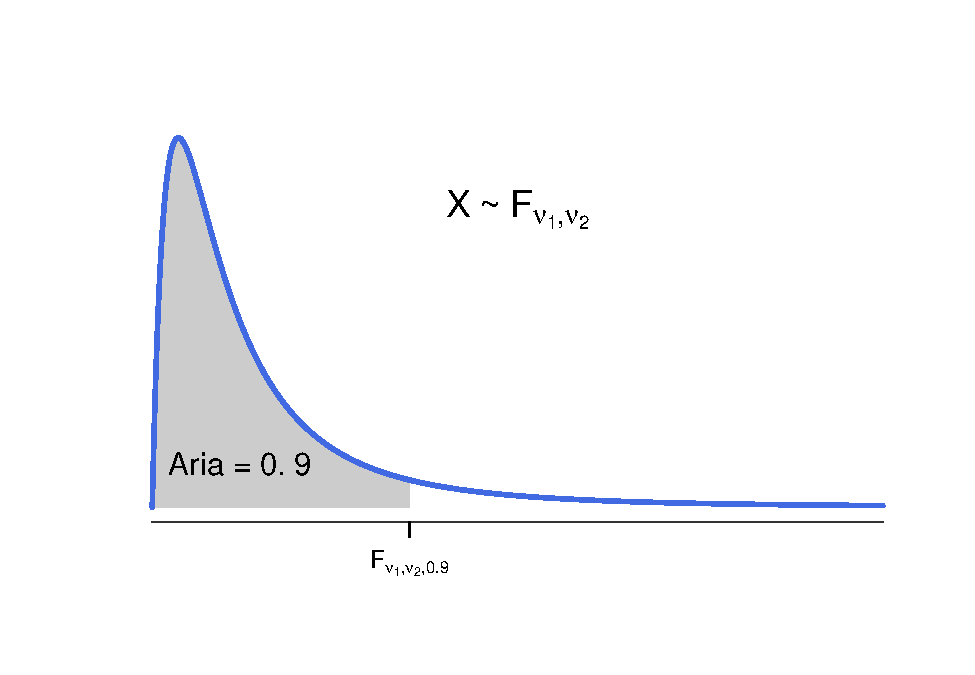
\includegraphics[width=0.4\linewidth]{Tabele_Statistice_files/figure-latex/unnamed-chunk-10-1} \end{center}

\begin{landscape}\begingroup\fontsize{5}{7}\selectfont
\rowcolors{2}{gray!6}{white}

\begin{longtable}{>{\bfseries}r|rrrrrrrrrrrrrrrrrrr}
\hiderowcolors
\toprule
$\nu_2 / \nu_1$ & 1 & 2 & 3 & 4 & 5 & 6 & 7 & 8 & 9 & 10 & 12 & 15 & 20 & 24 & 30 & 40 & 60 & 120 & $\infty$\\
\midrule
\endfirsthead
\multicolumn{20}{@{}l}{\textit{(continued)}}\\
\toprule
$\nu_2 / \nu_1$ & 1 & 2 & 3 & 4 & 5 & 6 & 7 & 8 & 9 & 10 & 12 & 15 & 20 & 24 & 30 & 40 & 60 & 120 & $\infty$\\
\midrule
\endhead
\
\endfoot
\bottomrule
\endlastfoot
\showrowcolors
1 & 39.864 & 49.500 & 53.593 & 55.833 & 57.240 & 58.204 & 58.906 & 59.439 & 59.858 & 60.195 & 60.705 & 61.220 & 61.740 & 62.002 & 62.265 & 62.529 & 62.794 & 63.061 & 63.328\\
2 & 8.526 & 9.000 & 9.162 & 9.243 & 9.293 & 9.325 & 9.349 & 9.367 & 9.380 & 9.392 & 9.408 & 9.425 & 9.441 & 9.450 & 9.458 & 9.466 & 9.475 & 9.483 & 9.491\\
3 & 5.538 & 5.462 & 5.391 & 5.343 & 5.309 & 5.285 & 5.266 & 5.252 & 5.240 & 5.230 & 5.216 & 5.200 & 5.184 & 5.176 & 5.168 & 5.160 & 5.151 & 5.143 & 5.134\\
4 & 4.545 & 4.325 & 4.191 & 4.107 & 4.051 & 4.010 & 3.979 & 3.955 & 3.936 & 3.920 & 3.896 & 3.870 & 3.844 & 3.831 & 3.817 & 3.804 & 3.790 & 3.775 & 3.761\\
5 & 4.060 & 3.780 & 3.619 & 3.520 & 3.453 & 3.405 & 3.368 & 3.339 & 3.316 & 3.297 & 3.268 & 3.238 & 3.207 & 3.191 & 3.174 & 3.157 & 3.140 & 3.123 & 3.105\\
\addlinespace
6 & 3.776 & 3.463 & 3.289 & 3.181 & 3.107 & 3.055 & 3.014 & 2.983 & 2.958 & 2.937 & 2.905 & 2.871 & 2.836 & 2.818 & 2.800 & 2.781 & 2.762 & 2.742 & 2.722\\
7 & 3.589 & 3.257 & 3.074 & 2.961 & 2.883 & 2.827 & 2.785 & 2.752 & 2.725 & 2.703 & 2.668 & 2.632 & 2.595 & 2.575 & 2.555 & 2.535 & 2.514 & 2.493 & 2.471\\
8 & 3.458 & 3.113 & 2.924 & 2.806 & 2.726 & 2.668 & 2.624 & 2.589 & 2.561 & 2.538 & 2.502 & 2.464 & 2.425 & 2.404 & 2.383 & 2.361 & 2.339 & 2.316 & 2.293\\
9 & 3.360 & 3.006 & 2.813 & 2.693 & 2.611 & 2.551 & 2.505 & 2.469 & 2.440 & 2.416 & 2.379 & 2.340 & 2.298 & 2.277 & 2.255 & 2.232 & 2.208 & 2.184 & 2.159\\
10 & 3.285 & 2.925 & 2.728 & 2.605 & 2.522 & 2.461 & 2.414 & 2.377 & 2.347 & 2.323 & 2.284 & 2.244 & 2.201 & 2.178 & 2.155 & 2.132 & 2.107 & 2.082 & 2.055\\
\addlinespace
11 & 3.225 & 2.860 & 2.660 & 2.536 & 2.451 & 2.389 & 2.342 & 2.304 & 2.273 & 2.248 & 2.209 & 2.167 & 2.123 & 2.100 & 2.076 & 2.052 & 2.026 & 2.000 & 1.972\\
12 & 3.176 & 2.807 & 2.606 & 2.480 & 2.394 & 2.331 & 2.283 & 2.245 & 2.213 & 2.188 & 2.147 & 2.105 & 2.060 & 2.036 & 2.011 & 1.986 & 1.960 & 1.932 & 1.904\\
13 & 3.136 & 2.763 & 2.560 & 2.434 & 2.347 & 2.283 & 2.234 & 2.195 & 2.164 & 2.138 & 2.097 & 2.053 & 2.007 & 1.983 & 1.958 & 1.931 & 1.904 & 1.876 & 1.846\\
14 & 3.102 & 2.727 & 2.522 & 2.395 & 2.307 & 2.243 & 2.193 & 2.154 & 2.122 & 2.095 & 2.054 & 2.010 & 1.962 & 1.938 & 1.912 & 1.885 & 1.857 & 1.828 & 1.797\\
15 & 3.073 & 2.695 & 2.490 & 2.361 & 2.273 & 2.208 & 2.158 & 2.119 & 2.086 & 2.059 & 2.017 & 1.972 & 1.924 & 1.899 & 1.873 & 1.845 & 1.817 & 1.787 & 1.755\\
\addlinespace
16 & 3.048 & 2.668 & 2.462 & 2.333 & 2.244 & 2.178 & 2.128 & 2.088 & 2.055 & 2.028 & 1.985 & 1.940 & 1.891 & 1.866 & 1.839 & 1.811 & 1.782 & 1.751 & 1.718\\
17 & 3.026 & 2.645 & 2.437 & 2.308 & 2.218 & 2.152 & 2.102 & 2.061 & 2.028 & 2.001 & 1.958 & 1.912 & 1.862 & 1.836 & 1.809 & 1.780 & 1.751 & 1.719 & 1.686\\
18 & 3.007 & 2.624 & 2.416 & 2.286 & 2.196 & 2.130 & 2.079 & 2.038 & 2.005 & 1.977 & 1.933 & 1.887 & 1.837 & 1.810 & 1.783 & 1.754 & 1.723 & 1.691 & 1.657\\
19 & 2.990 & 2.606 & 2.397 & 2.266 & 2.176 & 2.109 & 2.058 & 2.017 & 1.984 & 1.956 & 1.912 & 1.865 & 1.814 & 1.787 & 1.759 & 1.730 & 1.699 & 1.666 & 1.631\\
20 & 2.975 & 2.589 & 2.380 & 2.249 & 2.158 & 2.091 & 2.040 & 1.998 & 1.965 & 1.937 & 1.892 & 1.845 & 1.794 & 1.767 & 1.738 & 1.708 & 1.677 & 1.643 & 1.607\\
\addlinespace
21 & 2.961 & 2.575 & 2.365 & 2.233 & 2.142 & 2.075 & 2.023 & 1.982 & 1.948 & 1.920 & 1.875 & 1.827 & 1.776 & 1.748 & 1.719 & 1.689 & 1.657 & 1.623 & 1.586\\
22 & 2.949 & 2.561 & 2.351 & 2.219 & 2.128 & 2.061 & 2.008 & 1.967 & 1.933 & 1.904 & 1.859 & 1.811 & 1.759 & 1.731 & 1.702 & 1.671 & 1.639 & 1.604 & 1.567\\
23 & 2.937 & 2.549 & 2.339 & 2.207 & 2.115 & 2.047 & 1.995 & 1.953 & 1.919 & 1.890 & 1.845 & 1.796 & 1.744 & 1.716 & 1.686 & 1.655 & 1.622 & 1.587 & 1.549\\
24 & 2.927 & 2.538 & 2.327 & 2.195 & 2.103 & 2.035 & 1.983 & 1.941 & 1.906 & 1.877 & 1.832 & 1.783 & 1.730 & 1.702 & 1.672 & 1.641 & 1.607 & 1.571 & 1.533\\
25 & 2.918 & 2.528 & 2.317 & 2.184 & 2.092 & 2.024 & 1.971 & 1.929 & 1.895 & 1.866 & 1.820 & 1.771 & 1.718 & 1.689 & 1.659 & 1.627 & 1.593 & 1.557 & 1.518\\
\addlinespace
26 & 2.909 & 2.519 & 2.308 & 2.175 & 2.082 & 2.014 & 1.961 & 1.919 & 1.884 & 1.855 & 1.809 & 1.760 & 1.706 & 1.677 & 1.647 & 1.615 & 1.581 & 1.544 & 1.504\\
27 & 2.901 & 2.511 & 2.299 & 2.166 & 2.073 & 2.005 & 1.952 & 1.909 & 1.874 & 1.845 & 1.799 & 1.749 & 1.695 & 1.666 & 1.636 & 1.603 & 1.569 & 1.531 & 1.491\\
28 & 2.894 & 2.503 & 2.291 & 2.157 & 2.064 & 1.996 & 1.943 & 1.900 & 1.865 & 1.836 & 1.790 & 1.740 & 1.685 & 1.656 & 1.625 & 1.593 & 1.558 & 1.520 & 1.478\\
29 & 2.887 & 2.495 & 2.283 & 2.149 & 2.057 & 1.988 & 1.935 & 1.892 & 1.857 & 1.827 & 1.781 & 1.731 & 1.676 & 1.647 & 1.615 & 1.583 & 1.547 & 1.509 & 1.467\\
30 & 2.881 & 2.489 & 2.276 & 2.142 & 2.049 & 1.980 & 1.927 & 1.884 & 1.849 & 1.819 & 1.773 & 1.722 & 1.667 & 1.638 & 1.607 & 1.573 & 1.538 & 1.499 & 1.456\\
\addlinespace
40 & 2.835 & 2.440 & 2.226 & 2.091 & 1.997 & 1.927 & 1.873 & 1.829 & 1.793 & 1.763 & 1.715 & 1.662 & 1.605 & 1.574 & 1.541 & 1.506 & 1.467 & 1.425 & 1.377\\
60 & 2.791 & 2.393 & 2.177 & 2.041 & 1.946 & 1.875 & 1.819 & 1.775 & 1.738 & 1.707 & 1.657 & 1.603 & 1.544 & 1.511 & 1.476 & 1.437 & 1.395 & 1.348 & 1.292\\
120 & 2.748 & 2.347 & 2.130 & 1.992 & 1.896 & 1.824 & 1.768 & 1.722 & 1.684 & 1.652 & 1.601 & 1.545 & 1.482 & 1.447 & 1.409 & 1.368 & 1.320 & 1.265 & 1.193\\
$\infty$ & 2.705 & 2.303 & 2.084 & 1.945 & 1.847 & 1.774 & 1.717 & 1.670 & 1.631 & 1.599 & 1.546 & 1.487 & 1.421 & 1.383 & 1.342 & 1.295 & 1.240 & 1.169 & 1.000\\*
\end{longtable}
\rowcolors{2}{white}{white}\endgroup{}
\end{landscape}

\subsection{\texorpdfstring{Cunatile pentru
\(F_{\nu_1, \nu_2, 0.95}\)}{Cunatile pentru F_\{\nu_1, \nu_2, 0.95\}}}\label{cunatile-pentru-f_nu_1-nu_2-0.95}

\begin{center}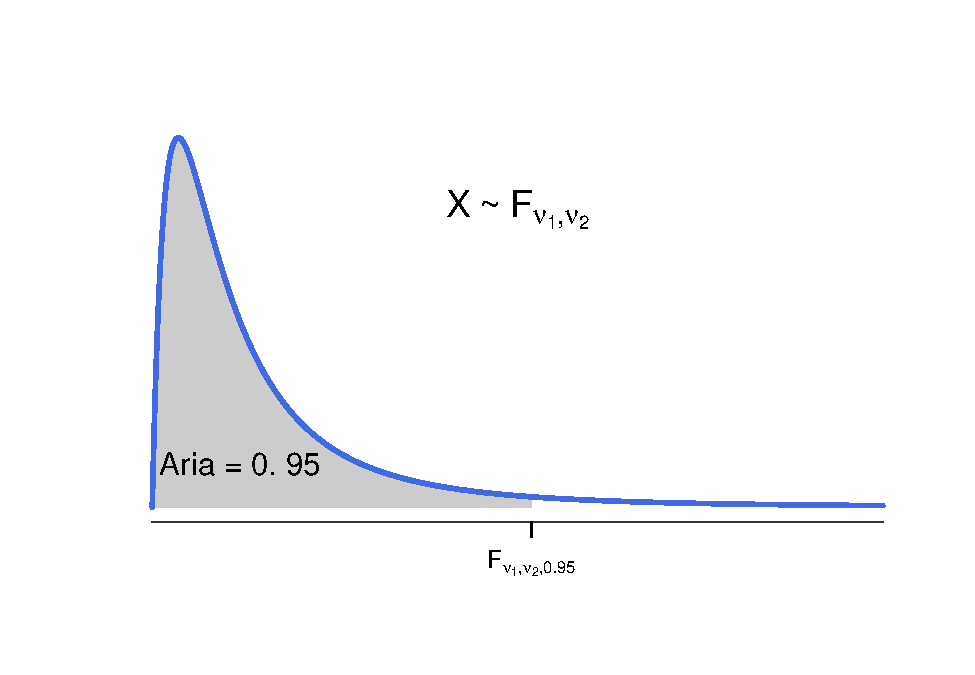
\includegraphics[width=0.4\linewidth]{Tabele_Statistice_files/figure-latex/unnamed-chunk-12-1} \end{center}

\begin{landscape}\begingroup\fontsize{5}{7}\selectfont
\rowcolors{2}{gray!6}{white}

\begin{longtable}{>{\bfseries}r|rrrrrrrrrrrrrrrrrrr}
\hiderowcolors
\toprule
$\nu_2 / \nu_1$ & 1 & 2 & 3 & 4 & 5 & 6 & 7 & 8 & 9 & 10 & 12 & 15 & 20 & 24 & 30 & 40 & 60 & 120 & $\infty$\\
\midrule
\endfirsthead
\multicolumn{20}{@{}l}{\textit{(continued)}}\\
\toprule
$\nu_2 / \nu_1$ & 1 & 2 & 3 & 4 & 5 & 6 & 7 & 8 & 9 & 10 & 12 & 15 & 20 & 24 & 30 & 40 & 60 & 120 & $\infty$\\
\midrule
\endhead
\
\endfoot
\bottomrule
\endlastfoot
\showrowcolors
1 & 161.45 & 199.50 & 215.71 & 224.58 & 230.16 & 233.99 & 236.77 & 238.88 & 240.54 & 241.88 & 243.91 & 245.95 & 248.01 & 249.05 & 250.09 & 251.14 & 252.20 & 253.25 & 254.31\\
2 & 18.51 & 19.00 & 19.16 & 19.25 & 19.30 & 19.33 & 19.35 & 19.37 & 19.39 & 19.40 & 19.41 & 19.43 & 19.45 & 19.45 & 19.46 & 19.47 & 19.48 & 19.49 & 19.50\\
3 & 10.13 & 9.55 & 9.28 & 9.12 & 9.01 & 8.94 & 8.89 & 8.85 & 8.81 & 8.79 & 8.74 & 8.70 & 8.66 & 8.64 & 8.62 & 8.59 & 8.57 & 8.55 & 8.53\\
4 & 7.71 & 6.94 & 6.59 & 6.39 & 6.26 & 6.16 & 6.09 & 6.04 & 6.00 & 5.96 & 5.91 & 5.86 & 5.80 & 5.77 & 5.75 & 5.72 & 5.69 & 5.66 & 5.63\\
5 & 6.61 & 5.79 & 5.41 & 5.19 & 5.05 & 4.95 & 4.88 & 4.82 & 4.77 & 4.74 & 4.68 & 4.62 & 4.56 & 4.53 & 4.50 & 4.46 & 4.43 & 4.40 & 4.37\\
\addlinespace
6 & 5.99 & 5.14 & 4.76 & 4.53 & 4.39 & 4.28 & 4.21 & 4.15 & 4.10 & 4.06 & 4.00 & 3.94 & 3.87 & 3.84 & 3.81 & 3.77 & 3.74 & 3.71 & 3.67\\
7 & 5.59 & 4.74 & 4.35 & 4.12 & 3.97 & 3.87 & 3.79 & 3.73 & 3.68 & 3.64 & 3.58 & 3.51 & 3.44 & 3.41 & 3.38 & 3.34 & 3.30 & 3.27 & 3.23\\
8 & 5.32 & 4.46 & 4.07 & 3.84 & 3.69 & 3.58 & 3.50 & 3.44 & 3.39 & 3.35 & 3.28 & 3.22 & 3.15 & 3.12 & 3.08 & 3.04 & 3.00 & 2.97 & 2.93\\
9 & 5.12 & 4.26 & 3.86 & 3.63 & 3.48 & 3.37 & 3.29 & 3.23 & 3.18 & 3.14 & 3.07 & 3.01 & 2.94 & 2.90 & 2.86 & 2.83 & 2.79 & 2.75 & 2.71\\
10 & 4.96 & 4.10 & 3.71 & 3.48 & 3.33 & 3.22 & 3.13 & 3.07 & 3.02 & 2.98 & 2.91 & 2.85 & 2.77 & 2.74 & 2.70 & 2.66 & 2.62 & 2.58 & 2.54\\
\addlinespace
11 & 4.84 & 3.98 & 3.59 & 3.36 & 3.20 & 3.10 & 3.01 & 2.95 & 2.90 & 2.85 & 2.79 & 2.72 & 2.65 & 2.61 & 2.57 & 2.53 & 2.49 & 2.45 & 2.40\\
12 & 4.75 & 3.88 & 3.49 & 3.26 & 3.11 & 3.00 & 2.91 & 2.85 & 2.80 & 2.75 & 2.69 & 2.62 & 2.54 & 2.50 & 2.47 & 2.43 & 2.38 & 2.34 & 2.30\\
13 & 4.67 & 3.81 & 3.41 & 3.18 & 3.02 & 2.92 & 2.83 & 2.77 & 2.71 & 2.67 & 2.60 & 2.53 & 2.46 & 2.42 & 2.38 & 2.34 & 2.30 & 2.25 & 2.21\\
14 & 4.60 & 3.74 & 3.34 & 3.11 & 2.96 & 2.85 & 2.76 & 2.70 & 2.65 & 2.60 & 2.53 & 2.46 & 2.39 & 2.35 & 2.31 & 2.27 & 2.22 & 2.18 & 2.13\\
15 & 4.54 & 3.68 & 3.29 & 3.06 & 2.90 & 2.79 & 2.71 & 2.64 & 2.59 & 2.54 & 2.48 & 2.40 & 2.33 & 2.29 & 2.25 & 2.20 & 2.16 & 2.11 & 2.07\\
\addlinespace
16 & 4.49 & 3.63 & 3.24 & 3.01 & 2.85 & 2.74 & 2.66 & 2.59 & 2.54 & 2.49 & 2.42 & 2.35 & 2.28 & 2.23 & 2.19 & 2.15 & 2.11 & 2.06 & 2.01\\
17 & 4.45 & 3.59 & 3.20 & 2.96 & 2.81 & 2.70 & 2.61 & 2.55 & 2.49 & 2.45 & 2.38 & 2.31 & 2.23 & 2.19 & 2.15 & 2.10 & 2.06 & 2.01 & 1.96\\
18 & 4.41 & 3.56 & 3.16 & 2.93 & 2.77 & 2.66 & 2.58 & 2.51 & 2.46 & 2.41 & 2.34 & 2.27 & 2.19 & 2.15 & 2.11 & 2.06 & 2.02 & 1.97 & 1.92\\
19 & 4.38 & 3.52 & 3.13 & 2.90 & 2.74 & 2.63 & 2.54 & 2.48 & 2.42 & 2.38 & 2.31 & 2.23 & 2.15 & 2.11 & 2.07 & 2.03 & 1.98 & 1.93 & 1.88\\
20 & 4.35 & 3.49 & 3.10 & 2.87 & 2.71 & 2.60 & 2.51 & 2.45 & 2.39 & 2.35 & 2.28 & 2.20 & 2.12 & 2.08 & 2.04 & 1.99 & 1.95 & 1.90 & 1.84\\
\addlinespace
21 & 4.33 & 3.47 & 3.07 & 2.84 & 2.68 & 2.57 & 2.49 & 2.42 & 2.37 & 2.32 & 2.25 & 2.18 & 2.10 & 2.05 & 2.01 & 1.97 & 1.92 & 1.87 & 1.81\\
22 & 4.30 & 3.44 & 3.05 & 2.82 & 2.66 & 2.55 & 2.46 & 2.40 & 2.34 & 2.30 & 2.23 & 2.15 & 2.07 & 2.03 & 1.98 & 1.94 & 1.89 & 1.84 & 1.78\\
23 & 4.28 & 3.42 & 3.03 & 2.80 & 2.64 & 2.53 & 2.44 & 2.38 & 2.32 & 2.27 & 2.20 & 2.13 & 2.05 & 2.00 & 1.96 & 1.91 & 1.86 & 1.81 & 1.76\\
24 & 4.26 & 3.40 & 3.01 & 2.78 & 2.62 & 2.51 & 2.42 & 2.35 & 2.30 & 2.25 & 2.18 & 2.11 & 2.03 & 1.98 & 1.94 & 1.89 & 1.84 & 1.79 & 1.73\\
25 & 4.24 & 3.38 & 2.99 & 2.76 & 2.60 & 2.49 & 2.40 & 2.34 & 2.28 & 2.24 & 2.16 & 2.09 & 2.01 & 1.96 & 1.92 & 1.87 & 1.82 & 1.77 & 1.71\\
\addlinespace
26 & 4.22 & 3.37 & 2.98 & 2.74 & 2.59 & 2.47 & 2.39 & 2.32 & 2.27 & 2.22 & 2.15 & 2.07 & 1.99 & 1.95 & 1.90 & 1.85 & 1.80 & 1.75 & 1.69\\
27 & 4.21 & 3.35 & 2.96 & 2.73 & 2.57 & 2.46 & 2.37 & 2.31 & 2.25 & 2.20 & 2.13 & 2.06 & 1.97 & 1.93 & 1.88 & 1.84 & 1.78 & 1.73 & 1.67\\
28 & 4.20 & 3.34 & 2.95 & 2.71 & 2.56 & 2.44 & 2.36 & 2.29 & 2.24 & 2.19 & 2.12 & 2.04 & 1.96 & 1.92 & 1.87 & 1.82 & 1.77 & 1.71 & 1.65\\
29 & 4.18 & 3.33 & 2.93 & 2.70 & 2.54 & 2.43 & 2.35 & 2.28 & 2.22 & 2.18 & 2.10 & 2.03 & 1.95 & 1.90 & 1.85 & 1.81 & 1.75 & 1.70 & 1.64\\
30 & 4.17 & 3.32 & 2.92 & 2.69 & 2.53 & 2.42 & 2.33 & 2.27 & 2.21 & 2.16 & 2.09 & 2.02 & 1.93 & 1.89 & 1.84 & 1.79 & 1.74 & 1.68 & 1.62\\
\addlinespace
40 & 4.08 & 3.23 & 2.84 & 2.61 & 2.45 & 2.34 & 2.25 & 2.18 & 2.12 & 2.08 & 2.00 & 1.92 & 1.84 & 1.79 & 1.74 & 1.69 & 1.64 & 1.58 & 1.51\\
60 & 4.00 & 3.15 & 2.76 & 2.52 & 2.37 & 2.25 & 2.17 & 2.10 & 2.04 & 1.99 & 1.92 & 1.84 & 1.75 & 1.70 & 1.65 & 1.59 & 1.53 & 1.47 & 1.39\\
120 & 3.92 & 3.07 & 2.68 & 2.45 & 2.29 & 2.17 & 2.09 & 2.02 & 1.96 & 1.91 & 1.83 & 1.75 & 1.66 & 1.61 & 1.55 & 1.50 & 1.43 & 1.35 & 1.25\\
$\infty$ & 3.84 & 3.00 & 2.60 & 2.37 & 2.21 & 2.10 & 2.01 & 1.94 & 1.88 & 1.83 & 1.75 & 1.67 & 1.57 & 1.52 & 1.46 & 1.39 & 1.32 & 1.22 & 1.00\\*
\end{longtable}
\rowcolors{2}{white}{white}\endgroup{}
\end{landscape}

\subsection{\texorpdfstring{Cunatile pentru
\(F_{\nu_1, \nu_2, 0.975}\)}{Cunatile pentru F_\{\nu_1, \nu_2, 0.975\}}}\label{cunatile-pentru-f_nu_1-nu_2-0.975}

\begin{center}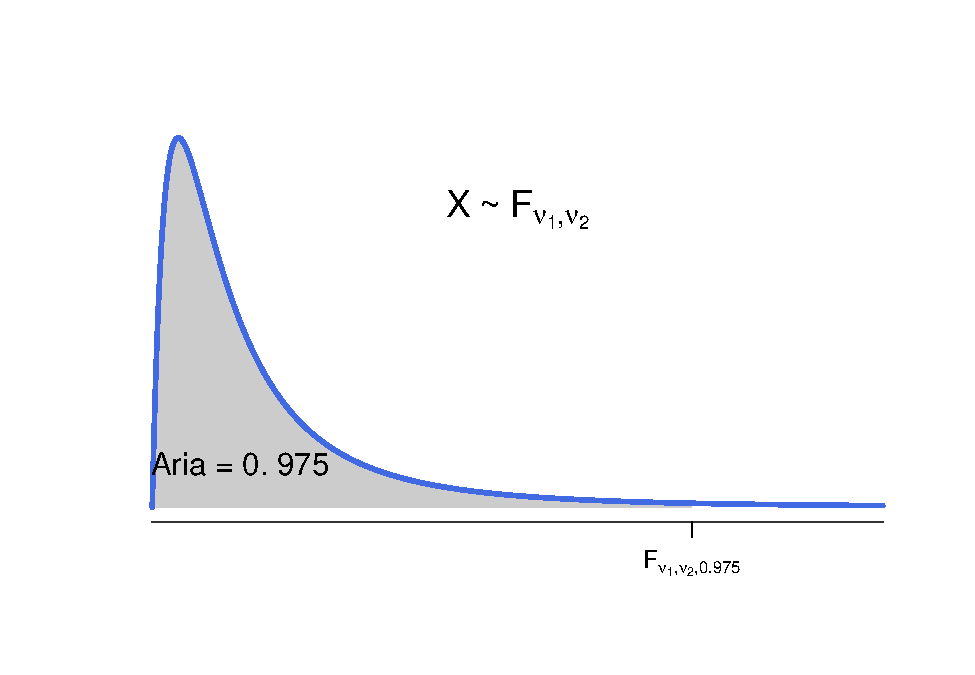
\includegraphics[width=0.4\linewidth]{Tabele_Statistice_files/figure-latex/unnamed-chunk-14-1} \end{center}

\begin{landscape}\begingroup\fontsize{5}{7}\selectfont
\rowcolors{2}{gray!6}{white}

\begin{longtable}{>{\bfseries}r|rrrrrrrrrrrrrrrrrrr}
\hiderowcolors
\toprule
$\nu_2 / \nu_1$ & 1 & 2 & 3 & 4 & 5 & 6 & 7 & 8 & 9 & 10 & 12 & 15 & 20 & 24 & 30 & 40 & 60 & 120 & $\infty$\\
\midrule
\endfirsthead
\multicolumn{20}{@{}l}{\textit{(continued)}}\\
\toprule
$\nu_2 / \nu_1$ & 1 & 2 & 3 & 4 & 5 & 6 & 7 & 8 & 9 & 10 & 12 & 15 & 20 & 24 & 30 & 40 & 60 & 120 & $\infty$\\
\midrule
\endhead
\
\endfoot
\bottomrule
\endlastfoot
\showrowcolors
1 & 647.79 & 799.50 & 864.16 & 899.58 & 921.85 & 937.11 & 948.22 & 956.66 & 963.28 & 968.63 & 976.71 & 984.87 & 993.10 & 997.25 & 1001.41 & 1005.60 & 1009.80 & 1014.02 & 1018.26\\
2 & 38.51 & 39.00 & 39.16 & 39.25 & 39.30 & 39.33 & 39.35 & 39.37 & 39.39 & 39.40 & 39.41 & 39.43 & 39.45 & 39.46 & 39.47 & 39.47 & 39.48 & 39.49 & 39.50\\
3 & 17.44 & 16.04 & 15.44 & 15.10 & 14.88 & 14.73 & 14.62 & 14.54 & 14.47 & 14.42 & 14.34 & 14.25 & 14.17 & 14.12 & 14.08 & 14.04 & 13.99 & 13.95 & 13.90\\
4 & 12.22 & 10.65 & 9.98 & 9.61 & 9.36 & 9.20 & 9.07 & 8.98 & 8.90 & 8.84 & 8.75 & 8.66 & 8.56 & 8.51 & 8.46 & 8.41 & 8.36 & 8.31 & 8.26\\
5 & 10.01 & 8.43 & 7.76 & 7.39 & 7.15 & 6.98 & 6.85 & 6.76 & 6.68 & 6.62 & 6.53 & 6.43 & 6.33 & 6.28 & 6.23 & 6.17 & 6.12 & 6.07 & 6.01\\
\addlinespace
6 & 8.81 & 7.26 & 6.60 & 6.23 & 5.99 & 5.82 & 5.70 & 5.60 & 5.52 & 5.46 & 5.37 & 5.27 & 5.17 & 5.12 & 5.07 & 5.01 & 4.96 & 4.90 & 4.85\\
7 & 8.07 & 6.54 & 5.89 & 5.52 & 5.29 & 5.12 & 5.00 & 4.90 & 4.82 & 4.76 & 4.67 & 4.57 & 4.47 & 4.42 & 4.36 & 4.31 & 4.25 & 4.20 & 4.14\\
8 & 7.57 & 6.06 & 5.42 & 5.05 & 4.82 & 4.65 & 4.53 & 4.43 & 4.36 & 4.29 & 4.20 & 4.10 & 4.00 & 3.95 & 3.89 & 3.84 & 3.78 & 3.73 & 3.67\\
9 & 7.21 & 5.71 & 5.08 & 4.72 & 4.48 & 4.32 & 4.20 & 4.10 & 4.03 & 3.96 & 3.87 & 3.77 & 3.67 & 3.61 & 3.56 & 3.50 & 3.45 & 3.39 & 3.33\\
10 & 6.94 & 5.46 & 4.83 & 4.47 & 4.24 & 4.07 & 3.95 & 3.85 & 3.78 & 3.72 & 3.62 & 3.52 & 3.42 & 3.37 & 3.31 & 3.25 & 3.20 & 3.14 & 3.08\\
\addlinespace
11 & 6.72 & 5.26 & 4.63 & 4.28 & 4.04 & 3.88 & 3.76 & 3.66 & 3.59 & 3.53 & 3.43 & 3.33 & 3.23 & 3.17 & 3.12 & 3.06 & 3.00 & 2.94 & 2.88\\
12 & 6.55 & 5.10 & 4.47 & 4.12 & 3.89 & 3.73 & 3.61 & 3.51 & 3.44 & 3.37 & 3.28 & 3.18 & 3.07 & 3.02 & 2.96 & 2.91 & 2.85 & 2.79 & 2.73\\
13 & 6.41 & 4.96 & 4.35 & 4.00 & 3.77 & 3.60 & 3.48 & 3.39 & 3.31 & 3.25 & 3.15 & 3.05 & 2.95 & 2.89 & 2.84 & 2.78 & 2.72 & 2.66 & 2.60\\
14 & 6.30 & 4.86 & 4.24 & 3.89 & 3.66 & 3.50 & 3.38 & 3.29 & 3.21 & 3.15 & 3.05 & 2.95 & 2.84 & 2.79 & 2.73 & 2.67 & 2.61 & 2.55 & 2.49\\
15 & 6.20 & 4.76 & 4.15 & 3.80 & 3.58 & 3.42 & 3.29 & 3.20 & 3.12 & 3.06 & 2.96 & 2.86 & 2.76 & 2.70 & 2.64 & 2.58 & 2.52 & 2.46 & 2.40\\
\addlinespace
16 & 6.12 & 4.69 & 4.08 & 3.73 & 3.50 & 3.34 & 3.22 & 3.12 & 3.05 & 2.99 & 2.89 & 2.79 & 2.68 & 2.62 & 2.57 & 2.51 & 2.45 & 2.38 & 2.32\\
17 & 6.04 & 4.62 & 4.01 & 3.66 & 3.44 & 3.28 & 3.16 & 3.06 & 2.98 & 2.92 & 2.83 & 2.72 & 2.62 & 2.56 & 2.50 & 2.44 & 2.38 & 2.31 & 2.25\\
18 & 5.98 & 4.56 & 3.95 & 3.61 & 3.38 & 3.22 & 3.10 & 3.00 & 2.93 & 2.87 & 2.77 & 2.67 & 2.56 & 2.50 & 2.44 & 2.38 & 2.32 & 2.26 & 2.19\\
19 & 5.92 & 4.51 & 3.90 & 3.56 & 3.33 & 3.17 & 3.05 & 2.96 & 2.88 & 2.82 & 2.72 & 2.62 & 2.51 & 2.45 & 2.39 & 2.33 & 2.27 & 2.20 & 2.13\\
20 & 5.87 & 4.46 & 3.86 & 3.52 & 3.29 & 3.13 & 3.01 & 2.91 & 2.84 & 2.77 & 2.68 & 2.57 & 2.46 & 2.41 & 2.35 & 2.29 & 2.22 & 2.16 & 2.08\\
\addlinespace
21 & 5.83 & 4.42 & 3.82 & 3.48 & 3.25 & 3.09 & 2.97 & 2.87 & 2.80 & 2.73 & 2.64 & 2.53 & 2.42 & 2.37 & 2.31 & 2.25 & 2.18 & 2.11 & 2.04\\
22 & 5.79 & 4.38 & 3.78 & 3.44 & 3.21 & 3.06 & 2.93 & 2.84 & 2.76 & 2.70 & 2.60 & 2.50 & 2.39 & 2.33 & 2.27 & 2.21 & 2.14 & 2.08 & 2.00\\
23 & 5.75 & 4.35 & 3.75 & 3.41 & 3.18 & 3.02 & 2.90 & 2.81 & 2.73 & 2.67 & 2.57 & 2.47 & 2.36 & 2.30 & 2.24 & 2.18 & 2.11 & 2.04 & 1.97\\
24 & 5.72 & 4.32 & 3.72 & 3.38 & 3.15 & 3.00 & 2.87 & 2.78 & 2.70 & 2.64 & 2.54 & 2.44 & 2.33 & 2.27 & 2.21 & 2.15 & 2.08 & 2.01 & 1.94\\
25 & 5.69 & 4.29 & 3.69 & 3.35 & 3.13 & 2.97 & 2.85 & 2.75 & 2.68 & 2.61 & 2.52 & 2.41 & 2.30 & 2.24 & 2.18 & 2.12 & 2.05 & 1.98 & 1.91\\
\addlinespace
26 & 5.66 & 4.26 & 3.67 & 3.33 & 3.10 & 2.94 & 2.82 & 2.73 & 2.65 & 2.59 & 2.49 & 2.39 & 2.28 & 2.22 & 2.16 & 2.09 & 2.03 & 1.95 & 1.88\\
27 & 5.63 & 4.24 & 3.65 & 3.31 & 3.08 & 2.92 & 2.80 & 2.71 & 2.63 & 2.57 & 2.47 & 2.36 & 2.25 & 2.19 & 2.13 & 2.07 & 2.00 & 1.93 & 1.85\\
28 & 5.61 & 4.22 & 3.63 & 3.29 & 3.06 & 2.90 & 2.78 & 2.69 & 2.61 & 2.55 & 2.45 & 2.34 & 2.23 & 2.17 & 2.11 & 2.05 & 1.98 & 1.91 & 1.83\\
29 & 5.59 & 4.20 & 3.61 & 3.27 & 3.04 & 2.88 & 2.76 & 2.67 & 2.59 & 2.53 & 2.43 & 2.33 & 2.21 & 2.15 & 2.09 & 2.03 & 1.96 & 1.89 & 1.81\\
30 & 5.57 & 4.18 & 3.59 & 3.25 & 3.03 & 2.87 & 2.75 & 2.65 & 2.58 & 2.51 & 2.41 & 2.31 & 2.19 & 2.14 & 2.07 & 2.01 & 1.94 & 1.87 & 1.79\\
\addlinespace
40 & 5.42 & 4.05 & 3.46 & 3.13 & 2.90 & 2.74 & 2.62 & 2.53 & 2.45 & 2.39 & 2.29 & 2.18 & 2.07 & 2.01 & 1.94 & 1.88 & 1.80 & 1.72 & 1.64\\
60 & 5.29 & 3.92 & 3.34 & 3.01 & 2.79 & 2.63 & 2.51 & 2.41 & 2.33 & 2.27 & 2.17 & 2.06 & 1.94 & 1.88 & 1.81 & 1.74 & 1.67 & 1.58 & 1.48\\
120 & 5.15 & 3.81 & 3.23 & 2.89 & 2.67 & 2.52 & 2.40 & 2.30 & 2.22 & 2.16 & 2.06 & 1.95 & 1.82 & 1.76 & 1.69 & 1.61 & 1.53 & 1.43 & 1.31\\
$\infty$ & 5.02 & 3.69 & 3.12 & 2.79 & 2.57 & 2.41 & 2.29 & 2.19 & 2.11 & 2.05 & 1.95 & 1.83 & 1.71 & 1.64 & 1.57 & 1.48 & 1.39 & 1.27 & 1.00\\*
\end{longtable}
\rowcolors{2}{white}{white}\endgroup{}
\end{landscape}


\end{document}
